%% GABARIT POUR THÈSE PAR ARTICLES
%%
%% Consulter la documentation de la classe ulthese pour une
%% description détaillée de la classe, de ce gabarit et des options
%% disponibles.
%%
%% [Ne pas hésiter à supprimer les commentaires après les avoir lus.]
%%
%% Déclaration de la classe avec le type de grade
%%   [l'un de LLD, DMus, DPsy, DThP, PhD]
%% et les langues les plus courantes. Le français sera la langue par
%% défaut du document. L'option 'bibsection' permet de créer des
%% bibliographies par chapitre présentées sous forme de section
%% numérotée.
\documentclass[PhD,bibsection,english,french]{ulthese}
  %% Encodage utilisé pour les caractères accentués dans les fichiers
  %% source du document. Les gabarits sont encodés en UTF-8. Inutile
  %% avec XeLaTeX, qui gère Unicode nativement.
  \ifxetex\else \usepackage[utf8]{inputenc} \fi

  %% Charger ici les autres paquetages nécessaires pour le document.
  %% Quelques exemples; décommenter au besoin.
  %\usepackage{amsmath}       % recommandé pour les mathématiques
  %\usepackage{ncccomma}      % gestion de la virgule dans les nombres

  %% Utilisation d'une autre police de caractères pour le document.
  %% - Sous LaTeX
  %\usepackage{mathpazo}      % texte et mathématiques en Palatino
  %\usepackage{mathptmx}      % texte et mathématiques en Times
  %% - Sous XeLaTeX
  %\setmainfont{TeX Gyre Pagella}      % texte en Pagella (Palatino)
  %\setmathfont{TeX Gyre Pagella Math} % mathématiques en Pagella (Palatino)
  %\setmainfont{TeX Gyre Termes}       % texte en Termes (Times)
  %\setmathfont{TeX Gyre Termes Math}  % mathématiques en Termes (Times)

  %% Gestion des hyperliens dans le document. S'assurer que hyperref
  %% est le dernier paquetage chargé.
  \usepackage{hyperref}
  \hypersetup{colorlinks,allcolors=ULlinkcolor}

  %% Options de mise en forme du mode français de babel. Consulter la
  %% documentation du paquetage babel pour les options disponibles.
  %% Désactiver (effacer ou mettre en commentaire) si l'option
  %% 'nobabel' est spécifiée au chargement de la classe.
  \frenchbsetup{%
    StandardItemizeEnv=true,       % format standard des listes
    ThinSpaceInFrenchNumbers=true, % espace fine dans les nombres
    og=«, fg=»                     % caractères « et » sont les guillemets
  }

  %% Suppression du numéro de section de la bibliographie. Utilisation
  %% de \extrasfrench parce que c'est la dernière langue déclarée dans
  %% \documentclass, ci-dessus.
  %\addto\extrasfrench{%
  %  \renewcommand{\bibsection}{\section*{\bibname}\prebibhook}}

  %% Déclarations des pages de titre. Remplacer les éléments entre < >.
  %% Supprimer les caractères < >. Couper un long titre ou un long
  %% sous-titre manuellement avec \\.
  \titre{<Titre principal>}
  % \titre{Ceci est un exemple de long titre \\
  %   avec saut de ligne manuel}
  % \soustitre{Sous-titre le cas échéant}
  % \soustitre{Ceci est un exemple de long sous-titre \\
  %   avec saut de ligne manuel}
  \auteur{<Prénom Nom>}
  \annee{<20xx>}
  \direction{<Prénom Nom>, <directeur ou directrice> de recherche}
  % \codirection{<Prénom Nom>, <codirecteur ou codirectrice> de recherche}
  % \codirection{<Prénom Nom>, <codirecteur ou codirectrice> de recherche \\
  %              <Prénom Nom>, <codirecteur ou codirectrice> de recherche}

\begin{document}

\frontmatter                    % pages liminaires

\pagestitre                     % production des pages de titre

\chapter*{Résumé}                      % ne pas numéroter
\phantomsection\addcontentsline{toc}{chapter}{Résumé} % inclure dans TdM

\begin{otherlanguage*}{french}
  Texte du résumé en français.
\end{otherlanguage*}
                % résumé français
\chapter*{Abstract}                      % ne pas numéroter
\phantomsection\addcontentsline{toc}{chapter}{Abstract} % inclure dans TdM

\begin{otherlanguage*}{english}

  Understanding images is needed for a plethora of tasks, from compositing to image relighting, including 3D object reconstruction. These tasks allow artists to realize masterpieces or help operators to safely make decisions based on visual stimuli. For many of these tasks, the physical and geometric models that the scientific community has developed give rise to ill-posed problems with several solutions, only one of which is generally reasonable. To resolve these indeterminations, the reasoning about the visual and semantic context of a scene is usually relayed to an artist or an expert who uses his experience to carry out his work. This is because humans are able to reason globally on the scene in order to obtain plausible and appreciable results. Would it be possible to model this experience from visual data and partly or totally automate tasks? This is the topic of this thesis: modeling priors using deep machine learning to solve typically ill-posed problems. More specifically, we will cover three research axes: 1) surface reconstruction using photometric cues, 2) outdoor illumination estimation from a single image and 3) camera calibration estimation from a single image with generic content. These three topics will be addressed from a data-driven perspective. Each of these axes includes in-depth performance analyses and, despite the reputation of opacity of deep machine learning algorithms, we offer studies on the visual cues captured by our methods. 

\end{otherlanguage*}
              % résumé anglais
\cleardoublepage

\tableofcontents                % production de la TdM
\cleardoublepage

\listoftables                   % production de la liste des tableaux
\cleardoublepage

\listoffigures                  % production de la liste des figures
\cleardoublepage

\dedicace{Dédicace si désiré}
\cleardoublepage

\epigraphe{Texte de l'épigraphe}{Source ou auteur}
\cleardoublepage

\chapter*{Remerciements}         % ne pas numéroter
\phantomsection\addcontentsline{toc}{chapter}{Remerciements} % inclure dans TdM

- HDRDB team
- Disney team
- Adobe team
         % remerciements
%!TEX root = main.tex
\chapter*{Preface}         % ne pas numéroter
\phantomsection\addcontentsline{toc}{chapter}{Preface} % inclure dans TdM

Most of the work presented in this dissertation was published in peer-reviewed conferences between 2015 and 2018 with myself as first author. %For every publication, I developed and executed all experiments, prepared the datasets and trained all machine learning models. 


Chapter~\ref{ch1} is mostly taken from our ICCP'15~\cite{holdgeoffroy-iccp-15} and 3DV'15~\cite{holdgeoffroy-3dv-15} publications. For the latter, we received the ``Best Paper (Runner Up)'' award in Lyon. More information on both works can be found on their project pages\footnote{\url{http://jflalonde.ca/projects/outdoorPS/} and \url{http://jflalonde.ca/projects/xHourPS/}}. The work presented on chapter~\ref{ch2} has been submitted for peer review at ECCV'18; we are still awaiting updates for this submission. Chapters~\ref{ch3} and~\ref{ch4} were both published to the prestigious CVPR (158 h-index), the former as a long oral presentation~\cite{holdgeoffroy-cvpr-17} (3\% acceptance rate), and the latter as a poster~\cite{holdgeoffroy-cvpr-18} (30\% acceptance rate). More information on both can be found on their project page\footnote{\url{http://jflalonde.ca/projects/deepOutdoorLight/} and \todo{add project page}}.


%\bibliographystyle{abbrvnat}
%\bibliography{library}
           % avant-propos

\mainmatter                     % corps du document

%%!TEX root = main.tex
\section{Introduction}

\begin{figure}
\centering
\includegraphics[width=\linewidth]{figures/teaser/teaser-skymodel.pdf}
\caption[Presentation of the proposed method]{We present an approach for predicting full HDR lighting conditions from a single LDR outdoor image. Our prediction can readily be used to insert a virtual object into the image. Our key idea is to train a CNN using input-output pairs of LDR images and HDR illumination parameters that are automatically extracted from a large database of $360^\circ$ panoramas.}
\label{fig:teaser}
\vspace{-1em}
\end{figure}

Illumination plays a critical role in deciding the appearance of a scene, and recovering scene illumination is important for a number of tasks ranging from scene understanding to reconstruction and editing. However, the process of image formation conflates illumination with scene geometry and material properties in complex ways and inverting this process is an extremely ill-posed problem. This is especially true in outdoor scenes, where we have little to no control over the capture process.

Previous approaches to this problem have relied on extracting cues such as shadows and shading~\cite{lalonde-ijcv-12} and combining them with (reasonably good) estimates of scene geometry to recover illumination. However, both these tasks are challenging and existing attempts often result in poor performance on real-world images. Alternatively, techniques for intrinsic images can estimate low-frequency illumination but rely on hand-tuned priors on geometry and material properties~\cite{barron-pami-15,lombardi2016reflectance} that may not generalize to large-scale scenes. In this work, we seek a single image outdoor illumination inference technique that generalizes to a wide range of scenes and does not make strong assumptions about scene properties.

To this end, our goal is to train a CNN to directly regress a single input low dynamic range image to its corresponding high dynamic range (HDR) outdoor lighting conditions. Given the success of deep networks at related tasks like intrinsic images~\cite{zhou2015intrinsic} and reflectance map estimation~\cite{rematas-cvpr-16}, our hope is that an appropriately designed CNN can learn this relationship. However, training such a CNN requires a very large dataset of outdoor images with their corresponding HDR lighting conditions. Unfortunately, such a dataset currently does not exist, and, because capturing light probes requires significant time and effort, acquiring it is prohibitive.

Our insight is to exploit a large dataset of outdoor panoramas~\cite{xiao-cvpr-12}, and extract photos with limited field of view from them. We can thus use pairs of photos and panoramas to train the neural network. However, this approach is bound to fail since: 1) the panoramas have low dynamic range and therefore do not provide an accurate estimate of outdoor lighting; and 2) even if notable attempts have been made~\cite{zhang-cvpr-13}, recovering full spherical panoramas from a single photo is both improbable and unnecessary for a number of tasks (e.g., many of the high-frequency details in the panoramas are not required when rendering Lambertian objects into the scene).

Instead, we use a physically-based sky model---the Ho\v{s}ek-Wilkie model~\cite{hosek-siggraph-12,hosek-cga-13}---and fit its parameters to the visible sky regions in the input panorama. This has two advantages: first, it allows us to recover physically accurate, high dynamic range information from the panoramas (even in saturated regions). Second, it compresses the panorama to a compact set of physically meaningful and representative parameters that can be efficiently learned by a CNN. At test time, we recover these parameters---including sun position, atmospheric turbidity, and geometric and radiometric camera calibration---from an input image and use them to construct an HDR sky environment map. 

To our knowledge, we are the first to address the complete scope of estimating a full HDR lighting representation---which can readily be used for image-based lighting~\cite{Debevec1998}---from a single outdoor image (fig.~\ref{fig:teaser}). Previous techniques have typically addressed only aspects of this problem, e.g., Lalonde et al.~\cite{lalonde-ijcv-12} recover the position of the sun but need to observe sky pixels in order to recover the atmospheric conditions. Similarly,~\cite{Ma2017} uses a neural network to estimate the sun azimuth to perform localization in roadside environments. Karsch et al.~\cite{karsch2014automatic} estimate full environment map lighting, but their panorama transfer technique may yield illumination conditions arbitrarily far away from the real ones. In contrast, our technique can recover an accurate, full HDR sky environment map from an arbitrary input image. We show through extensive evaluation that our estimates of the lighting conditions are significantly better than previous techniques and that they can be used ``as is'' to photorealistically relight and render 3D models into images.    



          % introduction
\chapter{Titre du chapitre}     % numéroté

Texte du chapitre.

\bibliographystyle{}              % style de la bibliographie
\bibliography{}                   % production de la bibliographie
    % chapitre 1
\chapter{Titre du chapitre}     % numéroté


%!TEX root = main.tex
\section{Introduction}

Despite nearly 40 years of study, the biggest challenge in outdoor Photometric Stereo (PS) remains the fact that the sun, our main light source, moves along a trajectory that nearly lies on a plane throughout the course of the day, leaving the photometric reconstruction under-constrained~\cite{woodham-opteng-80}.
%Researchers have investigated different approaches to address this problem, which include collecting data for several months~\cite{abrams-eccv-12,ackermann-cvpr-12}, waiting for the best time of the year (around summer solstice in the North Hemisphere~\cite{shen-pg-14}) or, more recently, for a day with favorable atmospheric conditions (partly cloudy sky~\cite{holdgeoffroy-iccp-15,holdgeoffroy-3dv-15}).
As previously discussed, one way to circumvent this issue is to wait for partially cloudy days for the effective lighting direction to shift away from the solar plane.
In general, the practitioner has no control over the sun or the atmosphere and is therefore left with two options: ($i$) a potentially long wait for the ideal conditions to arise; or ($ii$) the use of a smarter reconstruction technique that does not rely solely on the photometric cue.

In this chapter, we investigate the second option above. By using machine learning to aggregate prior knowledge on the geometry and reflectance of common classes of objects, we aim to resolve the ambiguities cause by the limited photometric cues available in single-day outdoor PS. To avoid restricting the algorithm to a small family of objects, we build knowledge on local geometry based on the fact that complex surfaces are made up of simpler, piecewise smooth patches. Our approach is further motivated by the fact that material properties are also locally correlated within small surface patches. Working with a broad class of small surface patches keeps the approach general and also facilitates the collection of data for machine learning.

% While non-convolutional deep learning was already used in fully-constrained, indoor PS (mostly to learn a generic, ``inverse BRDF'' function)... 

As we reason in terms of surface patches, a natural choice is to follow a deep learning approach with a novel convolutional neural network (CNN) architecture to automatically learn features from image patches and guide 3D normal estimation. To our knowledge, this is the first CNN to address the problem of under-constrained, single-day outdoor PS.

Our CNN design seeks a balance between fully-calibrated PS (too restrictive) and uncalibrated PS (which introduces further ambiguities). We follow a semi-calibrated outdoor PS approach and only assume that: (1) the object is imaged at roughly predefined times of the day; (2) the sun is unobstructed by clouds at these times; and (3) an orthographic camera facing approximately north (or south). The latter assumption could be relaxed using recent advances on sun position estimation in the wild to automatically detect the camera orientation. One could then train our model on multiple camera calibrations and select the right one according to the detected orientation. Of note, our approach does not require known sun intensities nor complete geolocation data, as in previous work on outdoor PS~\cite{jung-cvpr-15}. Together, our assumptions define an ``8-figure'' subspace for the position of the sun through the year, known as an {\em analemma}, whose shape also varies with geographical location (fig.~\ref{fig:solar-analemma}).

% (PG: that's an assummed/given condition)
% camera (pointing north, orthographic projection)

% analemma (Wikipedia): position of the Sun in the sky over the course of a year, as viewed at a fixed time of day and from a fixed location on the Earth

Therefore, our outdoor PS network is required to learn priors not only on object materials and local geometry (diffuse, specular, smooth, ...), but also priors on lighting (variability in sun intensity and elevation with respect to geolocation and time of year). This knowledge is encoded in the network, which learns to output 3D normals as a non-linear function of input image patches taken throughout a day. This rich prior knowledge allows us to obtain a reconstruction performance that outperforms the current state-of-the-art on real lighting data with only 3 images, which is much lower than the 6-18 typically used by previous work~\cite{yu-iccp-13,jung-cvpr-15}. Our fully trained method will be made publicly available.

%To train our CNN, we realistically render synthetic datasets with a large variety of image patches with different geometry, materials and lighting.

%\todo{Say something about the quality of our results vs state of the art.}

We summarize our contributions as follows:
\begin{itemize}
	\item a state-of-the-art method for single-day photometric stereo on sunny days that is robust to shadows, specularities and arbitrary but uniform albedo;
    \item a pipeline to generate synthetic images with a mix of Lambertian and glossy materials that captures the diversity of real outdoor lighting.
\end{itemize}


%!TEX root = main.tex
\section{Related work}

This section focuses on the more relevant work on outdoor PS, for conciseness. For an overview of general PS, the reader is referred to the recent, excellent review in~\cite{shi-tpami-18}.

% solar plane, nearly singular (ill-conditioned) light matrix, 2-image PS
% regularization breaks at (sharp) surface discontinuities

As shown in Woodham's seminal work~\cite{woodham-opteng-80}, for Lambertian surfaces, calibrated PS computes a (scaled) normal vector in closed form as a simple linear function of the input image pixels; this linear mapping is only well-defined for images obtained under three or more (known) non-coplanar lighting directions.
% webcams, solar plane
Subsequent work on outdoor PS has struggled to meet this requirement since, over the course of a day, the sun shines from directions that nearly lie on a plane. These co-planar sun directions then yield an ill-posed problem known as two-source PS; despite extensive research using integrability and smoothness constraints~\cite{onn-ijcv-90,hernandez-pami-11}, results still present strong regularization artifacts on surfaces that are not smooth everywhere. To avoid this problem in outdoor PS, authors initially proposed gathering months of data, watching the sun elevation change over the seasons~\cite{abrams-eccv-12,ackermann-cvpr-12}. More recently, Shen~{\em et al.}~\cite{shen-pg-14} noted that the coplanarity of the daily sun directions actually varies throughout the year, with single-day outdoor PS becoming more ill-posed at high latitudes near the winter solstice, and worldwide near the equinoxes.

% single day, ditch the even with a point light source model

% richer lighting models
To compensate for limited sun motion, other approaches use richer illumination models that account for additional atmospheric factors in the sky. This is done by employing (hemi-)spherical environment maps~\cite{debevec-siggraph-98} that are either real sky images~\cite{yu-iccp-13,shi-3dv-14,hung-wacv-15} or synthesized by parametric sky models~\cite{inose-tcva-13,jung-cvpr-15}. Using a large database of real sky images, Hold-Geoffroy~{\em et al.}~\cite{holdgeoffroy-iccp-15} showed that partly cloudy days are in fact better for single-day outdoor PS since clouds obscure and further scatter sun light, causing an out-of-plane shift in the effective direction of illumination. Subsequently~\cite{holdgeoffroy-3dv-15}, they also showed that good cloud coverage conditions for stable solutions may be observed in the sky within very short time intervals of just above one hour.

Despite these developments, state-of-the-art approaches in calibrated~\cite{yu-iccp-13} and semi-calibrated~\cite{jung-cvpr-15} (based on precise geolocation) outdoor PS are still prone to potentially long waits for ideal conditions to arise in the sky; and verifying the occurrence of such events is still a trial-and-error process. These facts have motivated our goal of developing a smarter approach that uses deep learning techniques to resolve ambiguities in outdoor PS by aggregating prior knowledge on object geometry, material and their interaction with natural outdoor illumination. The approach we propose is the first of its kind; so far, deep PS had only been applied in indoor scenarios with rich and controlled illumination~\cite{yu-iccv-17,santo-iccv-17,taniai-arxiv-18,shi-tpami-18}, focusing on learning inverse functions for non-Lambertian reflectances.

%\cite{yu-iccv-17,santo-iccv-17,taniai-arxiv-18} Deep learning methods applied to photometric stereo (not one-day)

% Talk about DiLiGent~\cite{shi-tpami-18}? (Their objects have homogeneous material, with piecewise constant albedo, our method would work with any albedo pattern using the division trick. Also, only normal maps, no 3D models. Their sampling of 96 lighting directions does not approximate well the path of the sun through a day.)

% single image (nishino, deep learning)
Finally, under more extreme ambiguity, techniques for shape-from-shading (SfS)~\cite{oxholm-eccv-12,johnson-cvpr-11,barron-pami-15} attempt to recover 3D normals from a single input image, in which case the shading cue alone is obviously insufficient to uniquely define a solution. Thus, SfS relies strongly on priors of different complexities and deep learning is quickly bringing advances to the field~\cite{eigen-iccv-15,shu-cvpr-17,wu-nips-17}. While this is encouraging, here we seek to improve the accuracy of 3D normal estimation by relying less heavily on priors and more strongly on the photometric cues obtained from multiple images. In addition, we also avoid restricting the approach to a specific type of object and reflectance model ({\em e.g.}, human faces, Lambertian~\cite{shu-cvpr-17}).

% deep learning PS and shape from shading, which rely on machine learning and priors, relate to original linear mapping in PS above.}
%
% This section could end by motivating the CNN: learning spatial priors is important.


% Move these to Sec 3-4 to further motivate CNN?
%
% Although there exists a closed-form least squares solution to the simplest Lambertian surfaces, such ideally diffuse materials rarely exist in the real word. Photometric stereo for surfaces with unknown general reflectance properties (i.e., bidirectional reflectance distribution functions or BRDFs) still remains as a fundamental challenge (Shi
%
% We know from data-driven, calibrated Lambertian PS that albedo and normals are obtained as a linear mapping from the input pixels. Here we relax the Lambertian and fully calibrated assumptions to learn a more generic, nonlinear mapping for recovering normal maps outdoors.
%
% Relate to 2-image PS problem early on? But that is for Lambertian case!
%
% Thus, 3D normal estimation based solely on the photometric cue remains under-constrained, even with strong assumptions of Lambertian reflectance and fully-calibrated illumination (the well-studied 2-image PS problem~\cite{}). 


%\section{Image formation model}

% Establish basic notation/formulation but only enough background as needed to support CNN-based method in next section...


% Linear and Lambertian assumptions
% We consider a small planar surface with normal vector $\mathbf{n} \in \mathbb{R}^3$ and Lambertian reflectance with albedo $\rho$. Under Lambertian assumption, all incoming lighting from the visible hemisphere can be formulated as a single point light source, the \emph{mean light vector} $\mathbf{\bar{l}­} \in \mathbb{R}^3$~\cite{holdgeoffroy-iccp-15,hung-wacv-15}.

% Given $m$ intensity observations of the same surface $b_1, b_2, ... b_m \in \mathbb{R}$ taken at different times of the day, yielding different mean light vectors $\mathbf{\bar{l}}_1, \mathbf{\bar{l}}_2, ... \mathbf{\bar{l}}_m \in \mathbb{R}^3$, we collect all photometric constraints for that pixel and obtain the PS equation in matrix form:
% \begin{equation}
%     \mathbf{b} = 
%     \begin{bmatrix}
%     b_1 \\
%     b_2 \\
%     \vdots \\
%     b_m
%     \end{bmatrix}
%     =
%     \begin{bmatrix}
%     \mathbf{\bar{l}}_1^T \\
%     \mathbf{\bar{l}}_2^T \\
%     \vdots \\
%     \mathbf{\bar{l}}_m^T
%     \end{bmatrix}
%     \mathbf{x}, = \rho\mathbf{Lx} \;,
% \label{eq:ifm}
% \end{equation}
% where $\mathbf{x} \in \mathbb{R}^3$ is the surface normal $\mathbf{n}$ scaled by the albedo $\rho$.

% The goal of PS is to recover the surface normal $\mathbf{n}$ from the pixel intensities $\mathbf{b}$ by solving eq.~\eqref{eq:ifm}. As discussed in~\cite{holdgeoffroy-3dv-15}, the uncertainty of the recovered surface normal is proportional to the conditioning of the lighting matrix $\mathbf{L}$.

% Throughout a clear day, the sun pursue a coplanar trajectory in the sky, yielding a poorly conditioned lighting matrix $\mathbf{L}$.

%\todo{Maybe we only briefly mention this in related work, unless the CNN builds on top of it (e.g., can we claim that often clouds cause small MLV shift, but still nearby the analema?). MLV implies Lambertian and we want to relax this limitation. Also, we have a directional light model now (don't we?), not a full envmap anymore.}

% 2-source PS is an approximation of single-day with Lambertian model, pt light

% \todo{Only add stuff that helps explain/motivate CNN in next section, so likely better to start writing Sec.4 first.}

% \todo{describe preliminaries for albedo division trick here?}

%!TEX root = main.tex
\section{Deep outdoor Photometric Stereo network}
\label{sec:proposed_method}

This section presents our CNN-based approach designed to address ambiguities that arise in single-day outdoor PS reconstruction. It does so by using deep learning to model prior knowledge on object geometry, material properties, as well as their local spatial correlation and interaction with natural sky light. In order to build such knowledge base, one needs a large number of images depicting various objects lit by outdoor lighting throughout the day, over different geographic locations and days over the year; finally, the surface normal map of each object is also required. Unfortunately, no such large-scale dataset currently exists, so a natural choice is to synthesize realistic data to train our network. We begin by presenting our problem formulation, CNN architecture, followed training procedure and data generation.

\subsection{Image formation model} % includes illumination subspace (analemmata)

% sky model can represent sun position, turbidity, etc... but not clouds, that's why we assume clear skies

% BRDF can be any family, we chose isotropic GGX which is popular these days...

Consider an image pixel that depicts a small area of an object's surface, with a normal vector ${\bf n} \in \Reals^3$ and material reflectance described by a bidirectional reflectance distribution function (BRDF) $\rho(\cdot)$. When viewed from direction \mbox{${\bf v} \in \Reals^3$}, the RGB color ${\bf b}_t \in \Reals^3$ of this pixel at daytime $t$ is modeled as
%
\begin{equation}
{\bf b}_t = \int_{\Omega_{\bf n}} \rho(\boldomega, {\bf v}, {\bf n}) {\bf  L}_t(\mathbf{\boldomega}) (\boldomega^T{\bf n}) V(\boldomega) d\omega \,,
\label{eq:ifm_singlepixel}
\end{equation}
%
where $\boldomega$ is a direction of incoming light within the hemispherical domain $\Omega_{\bf n}$, ${\bf L}_t(\mathbf{\boldomega})$ is the RGB intensities (color) of the incoming light at time $t$, and $V(\boldomega)$ is a binary visibility encoding self-shadowing. Here $t$ denotes the {\em actual solar time} at the target object location.

Our goal is to invert the above rendering equation and recover the surface normal ${\bf n}$ based on the observed changes in pixel intensities ${\bf b}_t$, which are caused by the changing natural illumination ${\bf L}_t(\mathbf{\boldomega})$ as $t$ varies throughout the day. However, as discussed above, a solution based solely on the photometric cue is rarely uniquely defined and stable in outdoor PS due to the limited motion of the sun, leading to insufficient variability in ${\bf L}_t(\mathbf{\boldomega})$ and, thus, ${\bf b}_t$~\cite{holdgeoffroy-3dv-15}.

Therefore, instead of considering a single pixel $\mathbf{b}_t$, we reformulate our goal and instead aggregate additional RGB image data within a \emph{neighborhood} ${\bf B}_t \in \Reals^{16 \times 16 \times 3}$, depicting a larger surface patch centered at the pixel $\mathbf{b}_t$. Now we seek to learn a predictor ${\bf N} = f({\bf B}_{t_1}, \ldots, {\bf B}_{t_T})$, where $T$ denotes the number of input images and ${\bf N} \in \Reals^{16\times 16\times 3}$ has the patch normals. For the present work, $T=8$ but we experiment with other values in sec.~\ref{sec:ablation_study}. This approach is motivated by the fact that complex object geometry is often made up of simpler, small surface patches presenting highly correlated surface normals and material properties. A natural way to obtain this predictor $f(\cdot)$ is to train a CNN that learns a nonlinear function of local surface features that are highly correlated with the normal ${\bf n}$ at the center of the patch. We train our network on a large synthetic database of surface patches realistically rendered with a standard GGX shader for $\rho(\cdot)$, with varying diffuse and specular parameters, and using the Ho\v{s}ek-Wilkie physically-based sky model~\cite{hosek-siggraph-12} for the spherical function ${\bf L}_t(\mathbf{\boldomega})$, as described next.

%\eqref{eq:ifm_singlepixel} is non-linear due to the reflectance function, and  and approximating the 2-source PS problem. Both issues can solved by learning priors that extend the photometric constraints.

% ambiguity, normals are locally correlated within a patch
% semi-calibrate, we don't require a light probe...
% assumptions... then architecture

% clouds, as long as don't obscure sun, change predominant direction of illumination considerably far from analemmata subsbace in Fig, should be ok. See experiments for sensitivity analysis.


\subsection{Illumination model: the solar analemma}
\label{sec:analemma}

We follow a semi-calibrated PS approach that does not require known lighting environments~\cite{yu-iccp-13} nor complete camera geolocation data~\cite{jung-cvpr-15}. Our method only assumes that: (1) the object images are captured at roughly predefined times of the day, $t \in \{t_1, t_2, \ldots, t_T \}$; (2) the sun is unobstructed by clouds at these times; and (3) the camera is orthographic and faces approximately North (or South). We later (sec.~\ref{sec:analysis}) analyze the robustness of our network with respect to departures from these ideal conditions and discuss how assumption~(3) can be relaxed.

Together, these assumptions constrain the sun position to lie within an ``8-figure'' subspace at each time $t$, known as a solar {\em analemma}, whose shape also varies with geographical location (fig.~\ref{fig:solar-analemma}). For a given time $t$, the sun may be positioned at different locations depending upon the selected date and latitude, as prescribed by the analemma. The neural network is thus expected to adapt to this (constrained) variability in sun position and associated intensity. As shown in fig.~\ref{fig:solar-analemma}-(a,b), for a given timestamp and latitude, the sun position spans relatively small angular ranges, which still remain quite constrained even when considering geographical locations sampled over the Northern Hemisphere (fig.~\ref{fig:solar-analemma}-(c)) (note that a similar plot would be obtained by sampling the Southern Hemisphere with the camera facing south). 

% On sunny days, illumination can change greatly depending on the geographical location of the observer and the date. On rare occasions, it can even provide sufficient contraints for photometric stereo~\cite{shen-pg-14}.

% One of the most notable effect is the solar analemma, namely the path of the sun in the sky throughout the year as viewed at a fixed time of day. Some analemmata like the ones shown in fig.~\ref{fig:sun_positions} exhibit over 45 degrees of azimuthal range through the year, especially early morning and late afternoon. This effect is different on the zenithal angle, where a variation similar in amplitude can be witnessed around noon. As the sun is the dominant light source on a sunny day, modeling this pattern can give hints to reason on the observed scene.

% This variability of the world over the course of a day is not accurately captured by currently available outdoor photometric stereo datasets. 

\begin{figure}[t]
    \centering
    \begin{tabular}{c@{\extracolsep{\fill}}cc}
        \includegraphics[width=0.34\linewidth]{figures/sun_pos/sunpos_paris.pdf} &
        \includegraphics[width=0.34\linewidth]{figures/sun_pos/sunpos_nt.pdf} &
        \makecell[t]{\includegraphics[width=0.29\linewidth]{figures/sun_pos/sunpos_all.pdf} \vspace{-5pt}\\
        \hspace{3pt}\includegraphics[width=0.22\linewidth]{figures/sun_pos/colorbar_sunpos_prob_horizontal.pdf}} \\
        \hspace{-11pt}(a) & \hspace{-11pt}(b) & \hspace{3pt}(c)
    \end{tabular} \\
    \caption[Solar analemma: position of the sun in the sky]{Solar analemma: position of the sun in the sky at a specific time of the day and throughout a year over (a) Paris and (b) the Tropic of Cancer. Note how the analemmas spread over a wide range of zenith and azimuth angles over the course of a year. (c)~Probability of the sun location in the sky for our training set.}
    \label{fig:solar-analemma}
\end{figure}

% Solar analemma: position of the Sun in the sky over the course of a year, as viewed at a fixed time of day and from a fixed location on the Earth

The physically-based parametric sky model of Ho\v{s}ek and Wilkie~\cite{hosek-siggraph-12} is used to obtain the spherical illumination function ${\bf L}_t(\mathbf{\boldomega})$ in eq.~\eqref{eq:ifm_singlepixel}. The model represents the spectral sky radiance as a parametric function of the sun position, sky turbidity and ground albedo. Here, turbidity is set to 2, which corresponds to a clear day, and ground albedo to 0.3. Note that we do not model light scattering caused by clouds obscuring the sun and thus assume the sun is fully visible in the sky.

\subsection{Network architecture}
\label{sec:architecture}

We now turn to the design of the function ${\bf N} = f({\bf B}_{t_1}, \ldots, {\bf B}_{t_T})$ introduced above, which is done through a Convolutional Neural Network (CNN). An overview of its proposed architecture is shown in fig.~\ref{fig:architecture}. The network takes $T=8$ input $16 \times 16$ image patches, extracted from 8 images captured at regular intervals $\Delta t$ between 9:00 and 16:00 solar time throughout a single sunny day. The first layer is composed of 32 channels of $5 \times 5$ filters with shared weights across the 8 inputs. The resulting feature maps are subsequently concatenated in a single $14 \times 14 \times 256$ feature tensor. A second convolutional layer is then used, yielding 256 channels, followed by 3 residual blocks as defined in the resnet-18 architecture~\cite{he-cvpr-16}. Lastly, 2 fully-connected layers (FC) are used to produce a $16 \times 16 \times 3$ patch of estimated normals $\mathbf{n}$. Note that we experimented with fully-convolutional architectures~\cite{taniai-arxiv-18} but found the FC layers to yield better results. The ELU activation function~\cite{clevert-iclr-16} is used at every convolutional and fully connected layer, except the output layer where a $\tanh(\cdot)$ function is used. Batch normalization~\cite{ioffe-icml-15} is applied at every layer except the first one and the output layer, where it could otherwise break low-level feature detectors and output distributions.

% The architecture mix of standard feed-forward convolutional and residual layers to learn the relationship between surface normals and photometric cues exhibited throughout a single day. 
% One particularity of our architecture is the large quantity of input heads of our CNN. 

\begin{figure}[t]
	\centering
	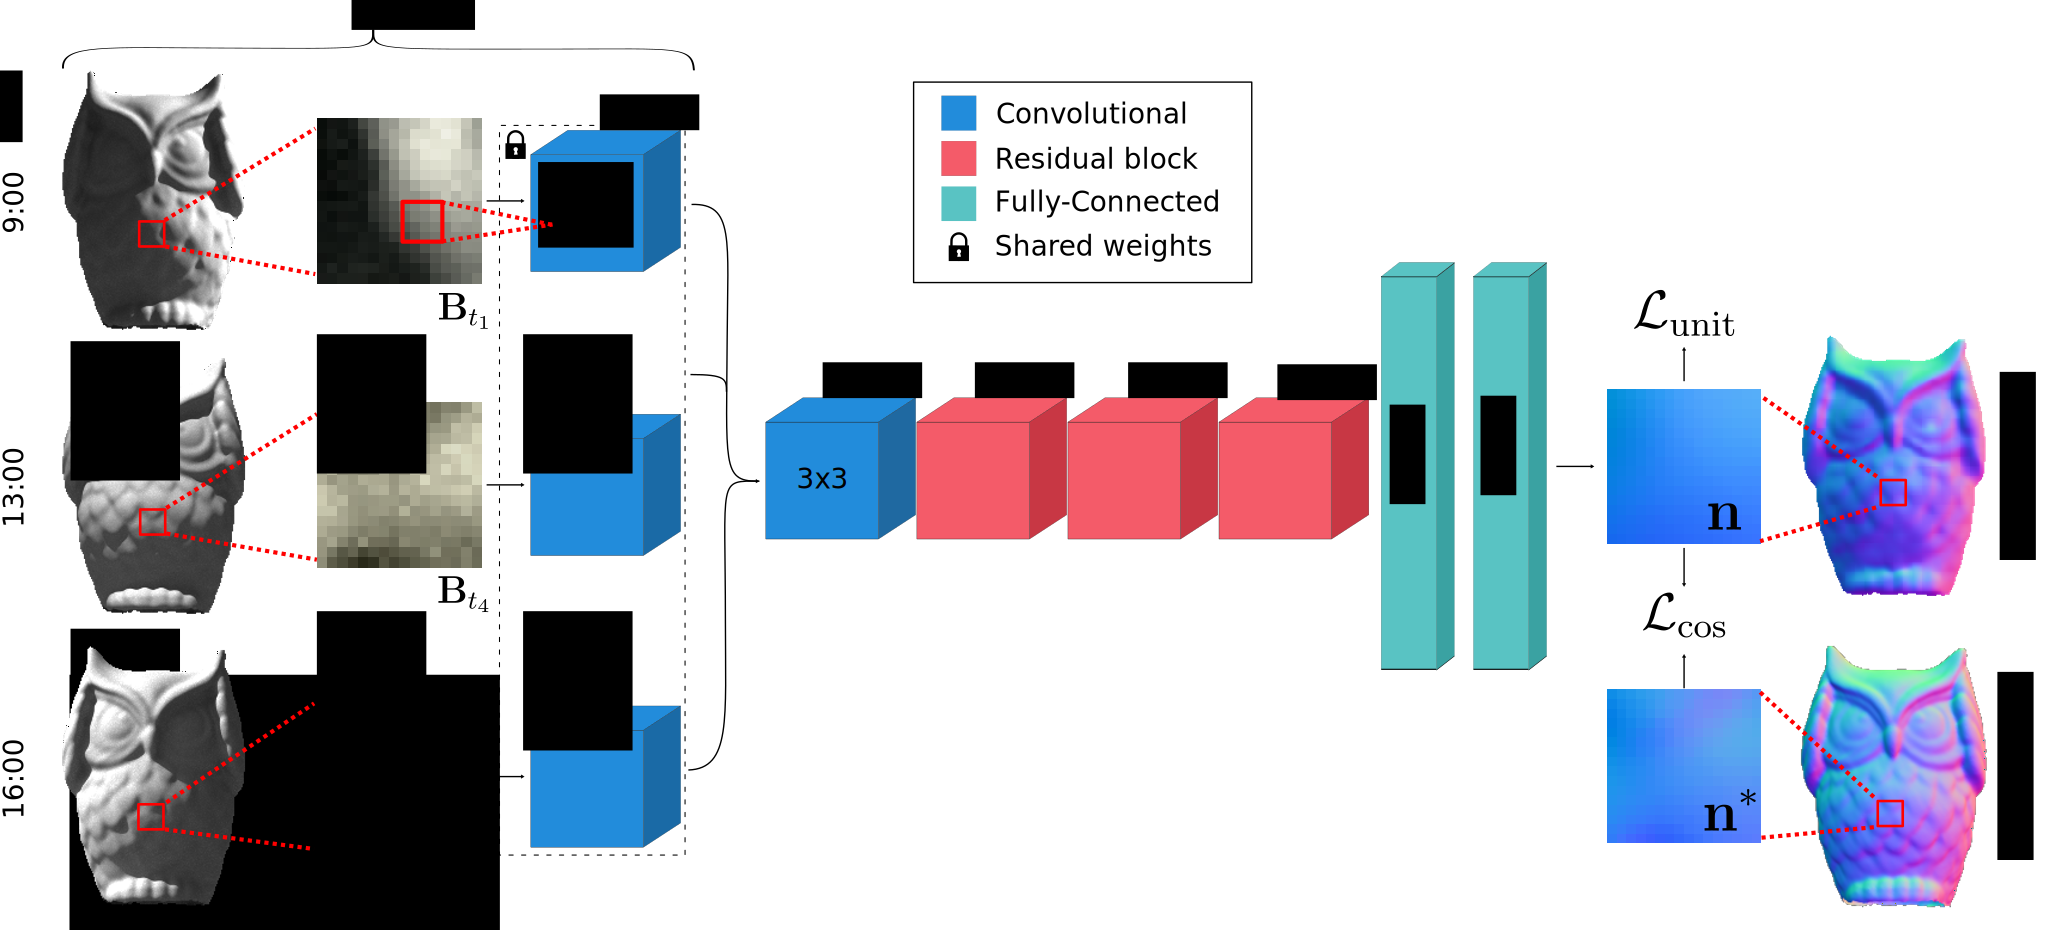
\includegraphics[width=0.8\linewidth]{figures/architecture.pdf}
	\caption[Method overview and model architecture]{Our novel CNN architecture for deep single-day outdoor PS on sunny days. The network operates on $16 \times 16$ patches $\mathbf{B}_t$ of the input image, captured at 8 time intervals $t$ regularly spaced throughout a single day. The network uses convolutional (blue) and residual (red) layers before estimating the normals using fully-connected layers (green). Two losses are used to train our method, one based on the cosine distance with the ground truth $\mathbf{\hat{n}}$ and another to constrain the norm of the output vector.}
	\label{fig:architecture}
\end{figure}

%, when photometric cues alone do not yield enough information for stable reconstruction. Using 8 input images captured at predefined times $t$ at regular intervals throughout a single sunny day, our convolutional architecture provides state-of-the-art results. We make two key observations: 1) spatial priors should be learned to overcome the weak conditioning induced by the single-day constraint, 2) to help generalization to new objects and limit the size of the training set, those spatial priors should be \emph{local}. 

The $16 \times 16$ estimated normals are represented by cartesian $(x,y,z)$ components of the surface normal of the input patch. We experimented with both cartesian $(x,y,z)$ and spherical coordinates $(\theta,\phi)$ parameterization, but found the cartesian parameterization to be more stable despite its additional degree of freedom. We hypothesize this may be due to the ``wrap-around'' issue with the azimuth angle $\phi$. 

To process entire images, we crop overlapping tiles from the image with a stride of 8 pixels. Since a pixel can belong to up to 4 patches, the network produces several estimates $\mathbf{\hat{n}}$ that are then merged together using a weighted average. We use a Gaussian kernel with $\sigma=4$ centered on the middle of the patch as weighting function to perform the linear interpolation across overlapping patches. %This weighted average is used as a normal estimation confidence, where we believe the normals estimated in the center of the patch to be of higher chance of being right as the CNN sees more context around them.

\subsection{Training}

The network learns a function that estimates the patch normals $\mathbf{N}$. We define the loss to be minimized between the estimated and ground truth patch normals $\mathbf{N}$ and $\mathbf{N}^*$ respectively as the sum of two separate loss functions defined on individual patch normals $\mathbf{n}_i$, $i \in \{1, ..., N\}$ where $N = 16 \times 16 = 256$. The total loss is the sum over all $N$ individual normals: 
%
\begin{equation}
\mathcal{L}(\mathbf{N}, \mathbf{N}^*) = \sum_{i=1}^{N} \left(\mathcal{L}_{\cos}(\mathbf{n}_i, \mathbf{n}^*_i) + \mathcal{L}_{\mathrm{unit}}(\mathbf{n}_i) \right)\,.
\label{eqn:loss}
\end{equation}
%
The first term is the cosine distance between the estimated $\mathbf{n}_i$ and ground truth normal $\mathbf{n}^*_i$:
%
\begin{equation}
\mathcal{L}_{\cos}(\mathbf{n}_i, \mathbf{n}^*_i) = 1 - \frac{ \left\langle \mathbf{n}_i , \mathbf{n}^*_i \right\rangle }{ \lVert \mathbf{n}_i \rVert \lVert \mathbf{n}^*_i \rVert } \,,
\end{equation}
%
where $\left\langle \cdot , \cdot \right\rangle$ denotes the dot product. The second term enforces the unit-length constraint on the recovered normal: 
%
\begin{equation}
\mathcal{L}_{\mathrm{unit}}(\mathbf{n}_i) = \left| \; \lVert \mathbf{n}_i \rVert - 1 \; \right| \,.
\end{equation}
%
The loss in eq.~\eqref{eqn:loss} is minimized via stochastic gradient descent using the Adam optimizer~\cite{kingma-iclr-15} with an initial learning rage of $\eta = 0.001$, a weight decay $\lambda = 1\times10^{-4}$ and the recommended values $\beta_1 = 0.9$ and $\beta_2 = 0.999$. Mini-batches of 128 samples were used during training and regularized via early stopping. Training typically converges in around 250 epochs on our dataset, which is described next.



% \begin{wrapfigure}{RLH}{0.5\textwidth}
% \vspace{-2em}
% \centering
% \includegraphics[width=\linewidth]{figures/training_step.png}
% \caption{Example of a validation step: 8th input (left), estimated normals $\mathbf{\hat{n}}$ (center) and ground truth normals $\mathbf{n}$ (right).}
% \label{fig:training_step}
% \vspace{-2em}
% \end{wrapfigure}


\subsection{Training dataset}
\label{sec:training_dataset}

To train our predictor function $f(\cdot)$, we rely on a large training dataset of synthetic objects, lit by a physically-based outdoor daylight model. To generate a single 8-images set of inputs, we randomly select a combination of: 1) object shape, 2) material properties, and 3) geo-temporal coordinates for lighting conditions. We now detail how each of these 3 choices are made. 

% Shape
Since the neural network only sees patches of $16 \times 16$ pixels, its receptive field is, by design, not large enough to learn priors on whole object shapes. Therefore, our dataset contains a wide variety of local surface curves. We used the blob dataset from~\cite{johnson-cvpr-11} as training models. We also added simple  primitives (cube, sphere, icosahedron, cone) to the dataset. A validation set, comprised of one of the blobs models that was kept from the training set as well as some models from the Stanford 3D Scanning Repository~\cite{curless-cg-96} and the owl model used in~\cite{holdgeoffroy-iccp-15}, was also created. All blobs and geometric primitives are randomly rotated about their centroid. 

% Materials

To model a wide range of surface appearance ranging from diffuse to glossy, we employ a linear combination of a lambertian and a microfacet model: 
%
\begin{equation}
\rho(\boldomega, {\bf v}, {\bf n}) = \boldrho_c (\alpha + (1-\alpha)\rho_\text{GGX}(\boldomega, {\bf v}, {\bf n}, \sigma)) \,,
\label{eq:brdf}
\end{equation}
%
where $\boldrho_c \in \Reals^3$ is the surface color, and $\rho_\text{GGX}$ is the GGX microfacet model~\cite{walter-eg-07} which is parameterized by the surface roughness $\sigma$. 

The albedo $\boldrho$ is generated in HSV space, where $H \sim U(0,1)$, $S \sim T(0, 0, 1)$, and $V \sim T(0, 0.75, 1)$, where $U(a, b)$ is a uniform distribution in the $[a, b]$ interval and $T(a,b,c)$ is a triangular distribution in the $[a,c]$ interval with mode $b$. This generates colors that are in general bright and prevents an abundance of strongly saturated colors. The surface roughness $\sigma$ is sampled as $\sigma \sim T(0.2, 0.4, 1)$ to avoid mirror-like surfaces. Finally, the mixing coefficient $\alpha$ is sampled as $\alpha \sim U(0,1)$. 

% Lighting
Accurately capturing outdoor illumination requires a carefully calibrated setup~\cite{stumpfel-afrigraph-04}, as such there exists limited number of real datasets (one notable exception being~\cite{hdrdb}). To light the scene with a wide variety of realistic outdoor lighting conditions, we instead rely on the Ho\v{s}ek-Wilkie physically-based sky model~\cite{hosek-siggraph-12} as described in sec.~\ref{sec:analemma}. We also placed a ground plane of albedo 0.3 outside the field of view of the camera, to generate a light bounce from below the object. 11 random locations in the Northern Hemisphere between latitude $0\degr$ (Equator) and $56\degr$ (Moscow) were selected. Furthermore, 6 random days throughout the year were chosen in addition to the equinoxes and solstices. This results in 110 pairs of geographical locations and dates, which are used to compute the sun position in the sky throughout the day using \cite{bretagnon-aaa-88}. The distribution of the resulting sun positions throughout our training set is shown in fig.~\ref{fig:solar-analemma}. For every pair of geographical location and day, 8 timestamps ranging from 9:00 to 16:00 are used to perform the renders. Timestamps are aligned to the solar noon instead of the political time zone of the geographic location. Note that, even though we sample only geographical locations in the northern hemisphere, our dataset represents equally well days in the southern hemisphere. Indeed, flipping the images left-right, reversing the image order (from 16:00 to 9:00) and pointing the camera southward would generate data identical to our training dataset.
%\todo{works at test time also?} => we never tested :(

% Stats
The resulting images are rendered with the Cycles physically-based rendering engine, effectively performing eq.~\eqref{eq:ifm_singlepixel} with the BRDF defined in eq.~\eqref{eq:brdf}. This results in a dataset of 369,440 renders corresponding to 23,090 combinations of geo-temporal coordinates and materials properties, which we then split into 21,220 and 1870 for training and validation, respectively. Each render has a resolution of $256 \times 256$ pixels, which amounts to over 10 millions input-output pairs of $16 \times 16$ patches to train on. Special care was taken into ensuring no 3D model nor material properties were shared between both the training and validation datasets. \textbf{Please consult the supplementary material for example training images obtained with this procedure}. 


%!TEX root = main.tex
\section{Evaluation}

\begin{figure}
\centering
\bgroup
\def\arraystretch{0}%  1 is the default, change whatever you need
\begin{tabular*}{\linewidth}{@{\hspace{1pt}}c@{\hspace{1pt}}c@{\hspace{1pt}}c@{\hspace{1pt}}c@{\hspace{1pt}}c@{\hspace{1pt}}c@{\hspace{1pt}}}

\vspace{2pt} 9:19 & 10:19 & 11:39 & 13:04 & 14:04 & 15:27 \\
\includegraphics[width=0.16\linewidth]{figures/results/examples/20130621/091938.png} &
%\includegraphics[width=0.2\linewidth]{figures/results/examples/20130621/094937.png} &
\includegraphics[width=0.16\linewidth]{figures/results/examples/20130621/101936.png} &
%\includegraphics[width=0.2\linewidth]{figures/results/examples/20130621/104435.png} &
%\includegraphics[width=0.2\linewidth]{figures/results/examples/20130621/111434.png} &
\includegraphics[width=0.16\linewidth]{figures/results/examples/20130621/113934.png} &
%\includegraphics[width=0.2\linewidth]{figures/results/examples/20130621/120933.png} &
%\includegraphics[width=0.2\linewidth]{figures/results/examples/20130621/123933.png} &
\includegraphics[width=0.16\linewidth]{figures/results/examples/20130621/130433.png} &
%\includegraphics[width=0.2\linewidth]{figures/results/examples/20130621/133432.png} &
\includegraphics[width=0.16\linewidth]{figures/results/examples/20130621/140431.png} &
%\includegraphics[width=0.2\linewidth]{figures/results/examples/20130621/144650.png} &
%\includegraphics[width=0.2\linewidth]{figures/results/examples/20130621/145704.png} &
\includegraphics[width=0.16\linewidth]{figures/results/examples/20130621/152700.png} \\%\includegraphics[width=0.2\linewidth]{figures/results/examples/20130621/155157.png} &
%\includegraphics[width=0.2\linewidth]{figures/results/examples/20130621/161154.png} \\

\includegraphics[width=0.16\linewidth]{figures/results/examples/20130621_inputs_owlie/img-01.png} &
\includegraphics[width=0.16\linewidth]{figures/results/examples/20130621_inputs_owlie/img-03.png} &
\includegraphics[width=0.16\linewidth]{figures/results/examples/20130621_inputs_owlie/img-06.png} &
\includegraphics[width=0.16\linewidth]{figures/results/examples/20130621_inputs_owlie/img-09.png} &
\includegraphics[width=0.16\linewidth]{figures/results/examples/20130621_inputs_owlie/img-11.png} &
\includegraphics[width=0.16\linewidth]{figures/results/examples/20130621_inputs_owlie/img-14.png} \\
\end{tabular*}

\noindent\rule{0.95\linewidth}{0.4pt}
\newcommand{\reswidth}{0.141}
\begin{tabular*}{\linewidth}{@{}c@{}c@{}c@{}c@{}c@{}c@{}c@{}}
\includegraphics[width=\reswidth\linewidth]{figures/results/examples/gt_owlie_normals.png} &
\includegraphics[width=\reswidth\linewidth]{figures/results/examples/ours_owlie_normals.png} &
\includegraphics[width=\reswidth\linewidth]{figures/results/examples/jung_owlie_normals.png} &
\includegraphics[width=\reswidth\linewidth]{figures/results/examples/yu_owlie_normals.png} &
\includegraphics[width=\reswidth\linewidth]{figures/results/examples/dpsn_owlie_normals.png} &
\includegraphics[width=\reswidth\linewidth]{figures/results/examples/marrnet_owlie_normals.png} &
\includegraphics[width=\reswidth\linewidth]{figures/results/examples/ef_owlie_normals.png} \\

\multicolumn{1}{r}{\includegraphics[height=\reswidth\linewidth]{figures/results/examples/colorbar_error_vertical.pdf}} &
\includegraphics[width=\reswidth\linewidth]{figures/results/examples/ours_owlie_errors.png} &
\includegraphics[width=\reswidth\linewidth]{figures/results/examples/jung_owlie_error.png} &
\includegraphics[width=\reswidth\linewidth]{figures/results/examples/yu_owlie_errors.png} &
\includegraphics[width=\reswidth\linewidth]{figures/results/examples/dpsn_owlie_errors.png} &
\includegraphics[width=\reswidth\linewidth]{figures/results/examples/marrnet_owlie_errors.png} &
\includegraphics[width=\reswidth\linewidth]{figures/results/examples/ef_owlie_errors.png} \\

\includegraphics[width=\reswidth\linewidth]{figures/results/examples/gt_buddha_normals.png} &
\includegraphics[width=\reswidth\linewidth]{figures/results/examples/ours_buddha_normals.png} &
\includegraphics[width=\reswidth\linewidth]{figures/results/examples/jung_buddha_normals.png} &
\includegraphics[width=\reswidth\linewidth]{figures/results/examples/yu_buddha_normals.png} &
\includegraphics[width=\reswidth\linewidth]{figures/results/examples/dpsn_buddha_normals.png} &
\includegraphics[width=\reswidth\linewidth]{figures/results/examples/marrnet_buddha_normals.png} &
\includegraphics[width=\reswidth\linewidth]{figures/results/examples/ef_buddha_normals.png} \\

\multicolumn{1}{r}{\includegraphics[height=\reswidth\linewidth]{figures/results/examples/colorbar_error_vertical.pdf}} &
\includegraphics[width=\reswidth\linewidth]{figures/results/examples/ours_buddha_errors.png} &
\includegraphics[width=\reswidth\linewidth]{figures/results/examples/jung_buddha_error.png} &
\includegraphics[width=\reswidth\linewidth]{figures/results/examples/yu_buddha_errors.png} &
\includegraphics[width=\reswidth\linewidth]{figures/results/examples/dpsn_buddha_errors.png} &
\includegraphics[width=\reswidth\linewidth]{figures/results/examples/marrnet_buddha_errors.png} &
\includegraphics[width=\reswidth\linewidth]{figures/results/examples/ef_buddha_errors.png} \\
\begin{tabular}{@{}c@{}}ground\\truth\end{tabular} & ours & \cite{jung-cvpr-15} & \cite{yu-iccp-13} & \cite{santo-iccv-17} & \cite{wu-nips-17} & \cite{eigen-iccv-15} \\
\end{tabular*}
\egroup
\caption[Lighting environment maps and renders throughout a day]{(top) An example of the lighting environment maps and renders throughout a day. (bottom) Qualitative results (odd rows) and errors in degrees (even rows) of our technique and the state-of-the-art on single-day photometric stereo in the semi-calibrated~\cite{jung-cvpr-15} and calibrated~\cite{yu-iccp-13} cases, deep photometric stereo~\cite{santo-iccv-17} and single image normal estimation~\cite{wu-nips-17,eigen-iccv-15} (averaged over the day) on our real lighting dataset. \textbf{More results available in annex~\ref{annex3}.}}
\label{fig:results-qualitative}
\end{figure}


In this section, we assess the performance of our method and compare it extensively to the state-of-the-art methods in single-day and regular photometric stereo, as well as some recent single image normal estimation techniques.

\subsection{Evaluation dataset}
\label{sec:evaluation_dataset}

To evaluate and compare the techniques, we rely on a dataset of synthetic objects, lit by real skies. To generate the images, we manually selected 3 sunny days over 2 geographical locations from the Laval HDR sky database~\cite{hdrdb}, which contains unsaturated HDR, omnidirectional photographs of the sky captured with the approach proposed in \cite{stumpfel-afrigraph-04}. We build a virtual 3D scene containing the HDR sky environment map as the sole light source, a 3D object viewed by an orthographic camera, and a 0.3 albedo ground plane placed under the object, outside the field of view of the camera. We used the 3D models from the validation set which the neural network never saw during training. This results in a dataset of 960 renders yielding 60 normal maps to evaluate. Example images obtained with this technique are shown in fig.~\ref{fig:results-qualitative}. 

% High dynamic range (HDR) captures of the sky hemisphere that span the full 22 stops required to properly capture outdoor lighting were taken using the approach proposed in~\cite{stumpfel-afrigraph-04}. We captured three different sunny days over two different geographical locations. 

%Days used: 2013-06-21 (Pittsburgh), 2015-05-14 and 2016-06-17 (Québec City). The sun has a maximum elevation of $73.00\degr$, $61.86\degr$ and $66.59\degr$, respectively.


\subsection{Results and comparisons}

We compare our method to several state-of-the-art techniques relying on photometric stereo and/or deep learning to estimate surface normals from images. For PS techniques, we compare to the calibrated technique of Yu et al.~\cite{yu-iccp-13}, which requires knowledge of the full environment map used to light the object. In our work, we use the variant proposed by Hold-Geoffroy et al.~\cite{holdgeoffroy-3dv-15} and without the low-rank matrix completion preprocessing, which was shown to yield slightly improved results over the original formulation. We also compare to the semi-calibrated method of Jung et al.~\cite{jung-cvpr-15}, which requires only knowledge of the capture geolocation. For deep learning techniques, we compare to the recent Deep Photometric Stereo Network (DPSN)~\cite{santo-iccv-17}, which operates on one pixel at a time. Since it assumes known point light source lighting, we re-trained this model using the sun position from a geographical location and date representative of our training dataset. In addition, we also compare to single image networks: Eigen and Fergus~\cite{eigen-iccv-15} and MarrNet~\cite{wu-nips-17}. Since they rely on a single image, we take the mean of their results averaged over all 8 inputs. 

The comparative results, shown qualitatively in fig.~\ref{fig:results-qualitative} and quantitatively in fig.~\ref{fig:results-quantitative}, clearly demonstrate that our approach significantly outperforms all other techniques. We observe that both single image techniques do not work well and result in very high median errors of around $40\degr$ and $70\degr$ for~\cite{wu-nips-17} and \cite{eigen-iccv-15}, respectively. For \cite{eigen-iccv-15}, this is probably due to the fact that they cannot handle the harsh shadows created by outdoor lighting during sunny days, since they train with indoor lighting only. In addition, MarrNet~\cite{wu-nips-17} outputs a voxel occupation grid and only produces normals as a byproduct (in its latent stage). As such, this method may not be fully optimized for normal estimation.

The PS techniques yield much better results but still yield quite significant error since sunny days do not contain sufficient constraints to accurately recover surface normals. The calibrated method of Yu et al.~\cite{yu-iccp-13} is comparable to the results obtained by DPSN, with a median normal angular estimation error of $33\degr$. Interestingly, the semi-calibrated method of Jung et al.~\cite{jung-cvpr-15} actually yields better results with a median error of $22\degr$, despite needing less information than the calibrated methods. This could be due to its reliance on a parametric clear sky model to estimate lighting, which closely matches the actual ground truth lighting, and to its reliance on an intensity profile matching algorithm.


\begin{figure}[t]
\centering
\includegraphics[width=0.75\linewidth]{figures/results/real_lighting_performance.pdf}
\caption[Reconstruction error on real lighting]{Median reconstruction error on our real lighting dataset displayed vertically as “box-percentile plots”~\cite{esty-jss-03}; the center horizontal bars indicate the median, while the bottom (top) bars are the 25th (75th) percentiles. Our proposed method (green) provides state-of-the-art performance compared to non-learned methods for single-day PS (blue~\cite{jung-cvpr-15}, orange~\cite{yu-iccp-13}), deep learning methods on calibrated photometric stereo (red~\cite{santo-iccv-17}) and single image normals reconstruction (purple~\cite{wu-nips-17}, brown~\cite{eigen-iccv-15}).}
\label{fig:results-quantitative}
\end{figure}

It is interesting to note that most PS techniques capture with some degree of success the left/right component of the surface normals (roughly speaking, the red and blue tints in the normal maps). This axis happens to be the same as the sun trajectory through the day when the camera is facing north or south. This results in strong photometric constraints on this axis. On the other hand, the recovery of the up/down axis is much less successful on most techniques as outdoor photometric cues lack information in this direction through a single sunny day.

In contrast, our method yields a normal map that is, although a bit smoother, qualitatively very similar to the ground truth. Quantitatively, our approach achieves a median error of $14\degr$ over the evaluation set, with the majority of errors being completely below that of the next-best performing method, Jung et al.~\cite{jung-cvpr-15} (see fig.~\ref{fig:results-quantitative}). Even if it is trained on purely synthetic data, our network is able to generalize well to images rendered with real lighting. The difference in performance with respect to DPSN shows the usefulness of dealing with image patches, which allows the network to learn appropriate patch-based shape priors which can be exploited when the photometric cue alone is not sufficient. 

% deep learning based photometric stereo~\cite{santo-iccv-17} as well as two recent single image normals estimation techniques: Eigen and Fergus~\cite{eigen-iccv-15} and MarrNet~\cite{wu-nips-17}. Qualitative results as well as quantitative results on median estimation error are shown in fig.~\ref{fig:experimental_results}-~\ref{fig:performance_real_lighting}, respectively. We observe that our proposed method outperforms previous work the vast majority of the time.


% Deep Photometric Stereo Network (DPSN)~\cite{santo-iccv-17} needs fully calibrated lighting positions. To evaluate on the one-day case, we trained this model using the sun position from a random geographical location and date. The model overfitted to this specific lighting pattern and did not adapt to different geographical locations and dates.

% In the case of~\cite{jung-cvpr-15}, the performance is reported on a subset of 2 objects over 2 days, and the MRF refinement post-processing was not performed. % Calibrated one-day photometric stereo~\cite{yu-iccp-13} was performed without the low-rank matrix completion preprocessing.

% ~\cite{yu-iccp-13,santo-iccv-17,jung-cvpr-15} all infer normals by looking at the photometric cues from a single pixel at a time. We argue that spatiality is important for one-day photometric stereo as it improves the signal-to-noise ratio in the axis perpendicular to the sun path through the day.



%\begin{figure}
%\centering
%\includegraphics[width=0.49\linewidth]{figures/analysis/perfs_per_direction_normal.pdf}
%\includegraphics[width=0.49\linewidth]{figures/analysis/perfs_per_direction_16divs.pdf}
%\hspace*{0.7cm}\begin{tabular*}{0.55\linewidth}{c@{\extracolsep{\fill}}c}
%(a) & (b)
%\end{tabular*} \\
%\caption{Reconstruction performance on our synthetic test dataset in function of the ground truth surface normal direction for our model with regular image input (a) and denominator images input (b).
%\todo{Should we keep this figure?}}
%\label{fig:surface_normal_direction}
%\end{figure}


%!TEX root = main.tex
\section{Analysis}
\label{sec:analysis}

We now analyze further our network, and in particular explore the robustness of our network to departures from the assumptions that were made in sec.~\ref{sec:proposed_method}. 

\subsection{Camera calibration error}

To constrain the set of possible lighting directions (sec.~\ref{sec:analemma}), we made the assumption that the camera is pointing north. We analyzed the impact on reconstruction performance when this hypothesis is infringed by rotating the real environment maps used to render the evaluation dataset (sec.~\ref{sec:evaluation_dataset}), and show the results of this experiment in fig.~\ref{fig:calibration_error_performance}. The slight improvement around $5\degr$ west calibration error is due to the timestamps of our real lighting dataset that are not perfectly aligned with the neural network expected timestamps. We observe that the median reconstruction error increases of approximately $5\degr$ per $10\degr$ error on camera calibration, showing that the network has some built-in robustness to these errors. 


\begin{figure}[!t]
\centering
\includegraphics[width=0.7\linewidth]{figures/analysis/performance_calibration_error.pdf}
\caption[Surface reconstruction performance in function of camera calibration error]{Median normal estimation error as box-percentile plots (see fig.~\ref{fig:results-quantitative}) in function of the camera deviation from north in degrees on our real lighting dataset. Positive means camera going toward west, negative means camera going toward east. }
\label{fig:calibration_error_performance}
\end{figure}


\subsection{Number of images}
\label{sec:ablation_study}

We now study the normal estimation performance in function of the number of inputs $T$ to the CNN (see sec.~\ref{sec:architecture}). Results ranging from a single input image ($T=1$, effectively performing shape-from-shading) to $T=16$ input images all uniformly taken from 9:00 to 16:00 are shown in fig.~\ref{fig:number_of_inputs}. We observe an rapid improvement in performance from one to three images, which is coherent with Photometric Stereo theory~\cite{woodham-opteng-80}. Performance continues to increase until $T=8$, probably because added constraints improves robustness to noise and non-diffuse materials. Interestingly, the normal estimation error starts to increase slightly with $T > 8$. This could be due to an increase in the number of parameters to train in our model (the output tensor after concatenation is of dimension $14 \times 14 \times 32T$, thereby increasing the number of parameters in the second convolutional layer), making the model harder to train.

% It is interesting to note the performance of the single image case, where the model obtains better than 24 degree median reconstruction error for half the renders, which is still quite competitive.


\begin{figure}[!t]
\centering
\includegraphics[width=0.75\linewidth]{figures/analysis/input_ablation.pdf}
\caption[Ablation study: surface reconstruction performance in function of the number of input images]{Median normal estimation error as box-percentile plots~\cite{esty-jss-03} (see fig.~\ref{fig:results-quantitative}) on our evaluation dataset as a function of $T$, the number of input images.}
\label{fig:number_of_inputs}
\end{figure}


\subsection{Feature analysis}

We use SmoothGrad~\cite{smilkov-arxiv-17} to visualize the regions of the image that have a larger impact on normal estimation. Since the network operates on patches and not entire images, we use the same linear blending strategy as in sec.~\ref{sec:training_dataset}, and report qualitative results in fig.~\ref{fig:smoothgrad}. We observe how the neural network tends to ignore darker regions and focuses on brighter alternatives in other images when available. This result suggests that the network learns to avoid shadowed areas, where, indeed, the photometric cue is not reliable due to low signal-to-noise ratio and to occlusion of the main light source.


\begin{figure}[!t]
\centering
\includegraphics[width=0.49\linewidth]{figures/analysis/smoothgrad_inputs.png}
\includegraphics[width=0.49\linewidth]{figures/analysis/smoothgrad.png} \\
\vspace{-1em}
\hspace*{-0.1cm}\begin{tabular*}{\linewidth}{c@{\extracolsep{\fill}}c}
 & \includegraphics[width=0.46\linewidth]{figures/analysis/colorbar_smoothgrad_horizontal.pdf}
\end{tabular*} \\
\vspace{-0.7em}
\hspace*{0.4cm}\begin{tabular*}{0.53\linewidth}{c@{\extracolsep{\fill}}c}
(a) & (b)
\end{tabular*} \\
\caption[CNN focus analysis]{Back-propagating the gradient through our network using SmoothGrad~\cite{smilkov-arxiv-17} on the input images shown in (a) generates a map of the pixels that affects the most the normal estimation (b). Notice how the regions in shadow have generally less influence (blue) than regions in direct sunlight (yellow).}
\label{fig:smoothgrad}
\end{figure}


%!TEX root = main.tex
\section{Discussion}



% % \begin{wrapfigure}{R}{0.5\textwidth}
\begin{figure}[!t]
% \centering
\floatbox[{\capbeside\thisfloatsetup{capbesideposition={left},capbesidewidth=6cm}}]{figure}[\FBwidth]
{
\begin{tabular}{c@{\extracolsep{\fill}}ccc}
\includegraphics[width=0.32\linewidth]{figures/results/uniform_output_crop.png} &
\includegraphics[width=0.32\linewidth]{figures/results/checker_normal_small_20160617_21_output_crop.png} &
\includegraphics[width=0.32\linewidth]{figures/results/checker_normal_large_20160617_21_output_crop.png} \\
%
\includegraphics[width=0.32\linewidth]{figures/results/uniform_input_gray_color_crop.png} &
\includegraphics[width=0.32\linewidth]{figures/results/checker_small_input_gray_color_crop.png} &
\includegraphics[width=0.32\linewidth]{figures/results/checker_large_input_gray_color_crop.png} 
\end{tabular}
}
{\caption{Limitation of our approach. Our network is trained on spatially uniform BRDFs, so testing it on spatially-varying albedo maps increases the estimation error. (left) Spatially-uniform albedos results in low error, while checkerboard albedo maps with (center) small and (right) large patterns increase the error.}\label{fig:limitations}}
\end{figure}


In this chapter, we present what we believe to be the first learned single-day photometric stereo method. Two key ideas were used to train our approach: first, local spatiality is important in the single-day case and can be leveraged using convolutional layers; second, large synthetic data with different surface reflectance can generalize well to real lighting and allows the training of deep learning methods. This results in a method robust to shadows, specular highlights and different albedos. We show that our method significantly outperforms previous work on a challenging evaluation dataset of virtual objects lit by real sunny lighting conditions.

Despite offering state-of-the-art performance, our method suffers from some limitations, which opens the way for interesting future work. The first limitation is that the camera is assumed to be pointing north. Although the network shows some resilience to errors in camera calibration (see fig.~\ref{fig:calibration_error_performance}), large deviations from the assumed direction are not well-handled. One possible way to circumvent this limitation would be to train direction-specific models and select the right one by detecting the camera orientation. Furthermore, while our approach is robust to non-Lambertian reflections, it assumes the scene to have a spatially-uniform BRDF. Fig.~\ref{fig:limitations} shows the behavior of our approach when the object is texture mapped with two spatially-varying albedo maps: a checkerboard pattern with small and large squares. Unsurprisingly, the resulting normal maps appear distorted since the constant albedo assumption is broken. One interesting direction for future work here would be to train a network on the \emph{ratio} between pairs of images (e.g. as in~\cite{yu-iccp-13}), which effectively cancels out the albedo. Lastly, we chose to focus on sunny days, since this is the most challenging case for outdoor photometric stereo~\cite{holdgeoffroy-iccp-15,holdgeoffroy-3dv-15}. Training the network on partially-cloudy days (for instance, by increasing the turbidity of the Ho\v{s}ek-Wilkie model) would be one potential way forward. 



% \section{Acknowledgements}




% To further understand the impact of non-uniform albedo on our approach, we applied a spatially-varying albedo to the the real lighting dataset used in evaluation. Two diffuse checkerboard patterns of different sizes were used as material. The checkerboard pattern sizes were chosen to be smaller and larger than the receptive field of our CNN. The dark squares from the checkerboard pattern have a gray albedo of 0.2 while the bright squares use the albedo sampling method described in sec.~\ref{sec:evaluation_dataset}. The results on this dataset are shown in fig.~\ref{fig:checker_experiments}. A loss of performance on the dataset median of roughly 3 and 5 degrees can be observe for the small and large checkerboard pattern, respectively. Qualitatively, our approach seems to assign a downward normal to the dark regions of the checkerboard pattern, as to explain the low pixel intensity by assuming it is facing the ground.




% \begin{figure}[!t]
% \centering
% \begin{tabular}{c@{\extracolsep{\fill}}ccc}
% \includegraphics[width=0.2\linewidth]{figures/results/uniform_output_crop.png} &
% \includegraphics[width=0.2\linewidth]{figures/results/checker_normal_small_20160617_21_output_crop.png} &
% \includegraphics[width=0.2\linewidth]{figures/results/checker_normal_large_20160617_21_output_crop.png} \\
% %
% \includegraphics[width=0.2\linewidth]{figures/results/uniform_input_gray_color_crop.png} &
% \includegraphics[width=0.2\linewidth]{figures/results/checker_small_input_gray_color_crop.png} &
% \includegraphics[width=0.2\linewidth]{figures/results/checker_large_input_gray_color_crop.png} \\
% (a) & (b) & (c)
% \end{tabular} \\
% \caption{Limitation of our approach. Our network is trained on spatially uniform BRDFs, so testing it on spatially-varying albedo maps increases the estimation error. (a) Quantiative comparison on our evaluation test set. (b) Spatially-uniform albedos results in low error, while checkerboard albedo maps with (c) small and (d) large patterns increase the error.}
% \label{fig:limitations}
% \end{figure}


% \begin{figure}[!t]
% \centering
% \begin{tabular}{c@{\extracolsep{\fill}}cccc}
% \multirow{2}{*}[4.5em]{\includegraphics[width=0.35\linewidth]{figures/results/checker_experiments.pdf}} &
% \includegraphics[width=0.2\linewidth]{figures/results/uniform_output.png} &
% \includegraphics[width=0.2\linewidth]{figures/results/checker_normal_small_20160617_21_output.png} &
% \includegraphics[width=0.2\linewidth]{figures/results/checker_normal_large_20160617_21_output.png} \\
% %
% & \includegraphics[width=0.2\linewidth]{figures/results/uniform_input_gray_color.png} &
% \includegraphics[width=0.2\linewidth]{figures/results/checker_small_input_gray_color.png} &
% \includegraphics[width=0.2\linewidth]{figures/results/checker_large_input_gray_color.png} \\
% (a) & (b) & (c) & (d)
% \end{tabular} \\
% \caption{Limitation of our approach. Our network is trained on spatially uniform BRDFs, so testing it on spatially-varying albedo maps increases the estimation error. (a) Quantiative comparison on our evaluation test set. (b) Spatially-uniform albedos results in low error, while checkerboard albedo maps with (c) small and (d) large patterns increase the error.}
% \label{fig:limitations}
% \end{figure}

% \begin{figure}[!t]
% \centering
% \begin{tabular}{c@{\extracolsep{\fill}}cccc}
% \multirow{2}{*}[4.5em]{\includegraphics[width=0.35\linewidth]{figures/results/checker_experiments.pdf}} &
% \includegraphics[width=0.18\linewidth]{figures/results/checker_20160617_21_gt.png} &
% \includegraphics[width=0.18\linewidth]{figures/results/checker_normal_small_20160617_21_output.png} &
% \includegraphics[width=0.18\linewidth]{figures/results/checker_normal_large_20160617_21_output.png} &
% \rotatebox[origin=l]{90}{\hspace{1.1em}normals} \\
% & \includegraphics[width=0.18\linewidth]{figures/results/checker_large_input.png} &
% \includegraphics[width=0.18\linewidth]{figures/results/checker_normal_small_20160617_21_error.png} &
% \includegraphics[width=0.18\linewidth]{figures/results/checker_normal_large_20160617_21_error.png} &
% \includegraphics[height=60pt]{figures/results/checker_colorbar_error_vertical.pdf}
% \rotatebox[origin=l]{90}{\hspace{2em}error} \\
% (a) & (b) & (c) & (d)
% \end{tabular} \\
% \caption{Evaluation on objects with non-uniform albedos. (a) Median reconstruction error in degrees of our method spatially uniform albedo maps (left), small and large checkerboard patterns (center and right) over our evaluation dataset. The ground truth normal map and example input image with a large checkerboard pattern are shown in (b). Qualitative normal recovery results and errors in degrees are shown for the small pattern (c) and large pattern (d).}
% \label{fig:checker_experiments}
% \end{figure}



\bibliographystyle{abbrvnat}
\bibliography{library}    % chapitre 2, etc.
%!TEX root = main.tex
\chapter*{Conclusion}         % ne pas numéroter
\phantomsection\addcontentsline{toc}{chapter}{Conclusion} % dans TdM


Throughout this thesis, we leverage the fact that gathering and analyzing large datasets can bring new insights that can both improve classical methods and build advanced machine learning algorithms. Three main axes of research were presented. First, we proposed a framework to analyze the performance of outdoor Photometric Stereo, which can explain the reasons leading to accurate tridimensional surface reconstruction through photometric signal under daylight. Using this framework, we demonstrated that partially cloudy days are more suited to perform outdoor PS from the photometric signal alone. We also showed that clear days typically do not yield enough photometric information to perform a robust surface reconstruction. We then presented a learning-based method that augments photometric cues with priors to solve the instability of the PS problem during sunny days. Secondly, we proposed a single image learning-based algorithm for outdoor lighting estimation that is robust to various scene content and exhibits state-of-the-art performance. We achieved this by fitting the physics-based Ho\v{s}ek-Wilkie sky model to a large dataset of 360$\degr$ panoramas and used it to train our machine learning model. Lastly, we used a similar approach to create a camera calibration method, which estimates automatically the field of view and the position of the horizon within the image. These last two methods can be used to streamline compositing operations by enabling automatic photorealistic virtual object insertion and relighting, along with applications like image retrieval. All proposed methods work on generic scenes and rely heavily on the priors modeled directly from the training data. 

For every project presented, we strove to understand the underlying patterns in the data. We proposed a framework for photometric stereo sensitivity analysis, which can predict reconstruction performance from the sky appearance. We also experimented with our surface reconstruction approach under various configurations to better understand the impact of camera calibration error and the number of input images on the reconstruction performance. Furthermore, the proposed camera calibration estimation method was analyzed through guided backpropagation, which allowed us to better understand the visual cues picked up by the learned model. Even though deep learning models are generally considered \emph{black boxes} by the community, we hope our efforts in explaining the behavior of those machine learning methods have inspired others to continue in this direction.

All approaches described in this thesis have direct applications in entertainment and advertisement, notably by enabling photorealistic virtual object insertion and relighting automatically. The lighting estimation and camera calibration techniques presented in this thesis (see chapters~\ref{ch3} and~\ref{ch4}) received worldwide recognition and were implemented into Dimension, the new 3D editing software from Adobe Systems. Thanks to these new technologies, multimedia artists are reporting their increased productivity and reduced time needed to create or modify works, as shown in the following testimony from a user: ``One of the greatest features is Dimension's ability to derive lighting from an image [and] use that to light an object. Results are amazing.'' In addition to its influence on digital media artists, the techniques proposed in this thesis also had an impact on the scientific community. We were selected to make an oral presentation at CVPR for our proposed lighting estimation method, a prestigious distinction (3\% acceptance rate in a conference holding an h-index impact score of 158). We also won the \emph{Best Paper (Runner Up)} award in 2015 at 3DV for the work presented in chapter~\ref{ch1}, which analyzed and improved outdoor surface reconstruction through photometric stereo. When applied outdoor, this technique can also have a large-scale impact, as it can be used to perform 3D scans of large statues and buildings, where hand-held scanning would take a prohibitive amount of time. The video game and movie industries use similar techniques to digitize actors~\cite{debevec2000acquiring} to produce photorealistic alter-egos. Using our proposed approach, the same could be done for large-scale elements like buildings and would allow studios to easily obtain high fidelity models for their creations. Aside from the entertainment industry, this technique can allow the preservation of cultural heritage of statues and buildings through digital copies that will stand the test of time. Additionally, the light and camera parameters estimation techniques we developed can also provide additional information to sensors, improving the quality of information provided by decision support systems. Similarly, our approaches could complement robot navigation and localization systems by providing another source of attitude estimation based on visual cues. Image forensics can also benefit from the ideas proposed in this thesis: detecting shadow orientations (by estimating sun position) and detecting conflicting horizons can help discover image modifications~\cite{Farid2010}. As can be seen, modeled priors can be used to perform hard computer vision tasks and have a myriad of applications.

Notwithstanding the advances proposed in this thesis, there are still some limitations to the presented approaches. For instance, the proposed method for outdoor surface reconstruction during sunny days expects the camera to point toward the north. A fully uncalibrated outdoor photometric stereo method has not yet been discovered. Also, while our lighting estimation method can predict accurately the sun position and most of the energy of the sky, it cannot model accurately its texture, as it models clouds as fog. Lastly, our proposed approach for camera calibration estimation does not support extreme pitch and roll angles due to the camera orientation representation we employed. We believe these limitations can be lifted in the foreseeable future by extending the approaches proposed in this thesis. On a broader note, it is our hope that this thesis has brought some insights and tools to enable the next generation of deep learned priors to computer vision tasks. 
            % conclusion

\appendix                       % annexes le cas échéant

\include{annexe}                % annexe A

\end{document}
